\documentclass[11pt]{article}
\usepackage[a4paper,margin=23mm]{geometry}
\usepackage[T1]{fontenc}
\usepackage{lmodern,amsmath,amssymb,amsthm,mathtools,microtype,graphicx,booktabs}
\usepackage[colorlinks=true,linkcolor=blue,citecolor=blue,urlcolor=blue]{hyperref}
\newcommand{\HH}{\mathcal H}
\newcommand{\Alg}{\mathcal A}
\newcommand{\K}{\mathcal K(\HH)}
\newcommand{\dd}{\mathrm d}
\newcommand{\norm}[1]{\left\lVert#1\right\rVert}
\newcommand{\E}{\mathbb E}
\newcommand{\NN}{\mathcal N}
\newtheorem{proposition}{Proposition}
\title{A same-disorder covariant channel in the Slater representation\\
\large Mixed words, a new cyclic direction and a stationary tracial sector}
\author{Alan Day \and Chengheng\thanks{AI research assistant (OpenAI).}}
\date{8 November 2026\quad Local research draft}
\begin{document}\maketitle
\begin{abstract}
We add a microscopic covariant size descendant of the Hamiltonian to
the selected Slater algebra. A marked-site extension of the normalized
CAR defect expansion gives all fixed mixed words and compact-time
convergence in the same Gaussian disorder. The new vector has a strictly
positive component outside the entire previous cyclic space. Its joint
transfer still has a compact selected operator, but a long-time state now
retains a noncommutative two-color $q$-Gaussian sector. We identify the GNS
representation of this particular stationary state, not the full
quotient algebra or every stationary state. The results concern the
specified annealed double-scaled model; the gravitational dictionary
remains to be constructed.
\end{abstract}

\section{Model and the constructive question}
The previous selected algebra contained only $h,M,M^\dagger$.
Its stationary states killed the compact selected channel and retained
only a commutative energy algebra. We now enlarge the microscopic
observable set before taking the limit. The fixed-charge chord
framework is established in \cite{BNR}; $q$-Gaussian Wick calculus in
\cite{EP}; the dependence of the representation on the chosen observable
algebra is central to \cite{RX,Xu}. Here the additional operator is a
descendant of the original random Hamiltonian, with its mixed
correlations derived in the selected state.

Use standard CAR, even $N$, $m=N/2$, a fixed occupied set $O$ and its
empty complement $E$. For ordered $p$-element subsets write
\begin{equation}
 H_N=\sqrt{w_N}\sum_{A,B}J_{AB}C_A^\dagger C_B,
 \qquad \E J_{AB}J_{CD}=\delta_{AD}\delta_{BC}.
\end{equation}
The matrix $J$ is Hermitian Gaussian; $A\cap B$ is allowed. Set
\begin{align}
 L_N&=\binom mp^2,& D_N&=\binom mp\binom{m+p}p,&
 h_N&=H_N/\sqrt{w_ND_N},\\
 M_N^\dagger&=L_N^{-1/2}
 \sum_{A\subset E,\,B\subset O}J_{AB}C_A^\dagger C_B,&
 \varphi_N(X)&=\E\langle O|X|O\rangle.
\end{align}
Both subset sizes in the last sum are $p$. Throughout,
$\lambda_N=p^2/N\to\lambda>0$, $q=e^{-4\lambda}$,
$\gamma=q^{1/4}$ and $s=\sqrt q$. Time is conjugate to dimensionless $h$;
the physical string energy is $(J_s/\sqrt\lambda)h$, with $\hbar=1$.

\newpage
\section{The microscopic descendant and marked local sources}
Let $\mathcal L$ denote full-Fock half-Clifford-size, acting on operators
before restriction to the central charge sector. Our new field is
\begin{equation}\label{eq:u}
 u_N=\frac{(p-\mathcal L-\lambda_N)h_N}{\sqrt{\lambda_N}}.
\end{equation}
It is Hermitian, linear in the same $J$, and $U(N)$-equivariant. It is the
normalized first size fluctuation used in the earlier bilocal expansion,
not an independent matter ensemble.

For $X=C_A^\dagger C_B$, an own-overlap site in $A\cap B$ contributes a
number operator $n$. At that site $p-\mathcal L$ replaces $n$ by $I/2$;
one sums over all own-overlap sites. Equivalently, its exponential
replaces $n$ by $n+(e^z-1)I/2$. Give each differentiated endpoint a
commuting nilpotent source $z_i$, $z_i^2=0$. The local replacement is
then exactly $n+z_iI/2$. Single-membership sites have no source.

Retain the fixed empty/occupied Slater CAR factors and the Jordan signs
from the previous site polynomial. For an unrestricted Gaussian edge
with endpoints $i,j$, its own two-label collision, summed over empty and
occupied sites, has polynomial
\begin{equation}\label{eq:local}
 1+\tfrac12 z_i+\tfrac12 z_j+\tfrac12 z_i z_j.
\end{equation}
The constant term comes from the occupied site. The two linear terms
each give $\langle n/2\rangle$; the quadratic term gives $1/4$ on both
occupations. A selected edge forbids this own overlap. Double membership
belonging to two different edges has no source: neither endpoint has
both labels of its own edge at that site. Higher memberships will be
controlled after normalization, rather than discarded by an
unnormalized rarity argument.

Centering the endpoint by $-\lambda_N$ multiplies its source by
$e^{-\lambda_N z_i}$. The activity of a double cluster tends to
$m(p/m)^2=2\lambda$. Thus the source-dependent exponent from
\eqref{eq:local} is
$\lambda(z_i+z_j)+\lambda z_i z_j$. After centering, an unrestricted
edge has source $e^{\lambda z_i z_j}$. A selected edge with a
differentiated unrestricted endpoint has instead $e^{-\lambda z_i}$.
Dividing each derivative by $\sqrt\lambda$ gives the edge coefficients
\begin{equation}\label{eq:coeff}
 w(H,H)=w(U,U)=1,\quad w(H,U)=0,\quad
 w(H,P)=\gamma,\quad w(U,P)=-\sqrt\lambda\,\gamma.
\end{equation}
Here $P$ denotes the selected endpoint of a compatible edge; an edge
with two selected endpoints has weight one. Its orientation restriction
is unchanged. The derivation of the $U$--selected coefficient is
especially important: tracial orthogonality of $h$ and $u$ does not
imply orthogonality to $M^\dagger$ in the selected state.

\newpage
\section{Normalized defect proof of the all-word limit}
Fix a word of length $2k$ and one Gaussian pairing. An edge is
unrestricted ($G$) if neither endpoint is selected; otherwise its label
is restricted by the selected endpoint(s). For each occupation
$o\in\{0,1\}$, let $n_{o,S}$ count sites with membership subset $S$ of
the $2k$ edge labels, $|S|\ge2$. Define the deficits
$d_i=\sum_{o,S\ni i}n_{o,S}$, so the remaining singleton count is $p-d_i$.
The exact normalized coefficient, divided by $L_N^k$, has terms
\begin{equation}\label{eq:defect}
 \frac{(m)_{V_0}(m)_{V_1}}{(m)_p^{2k}}
 \prod_i(p)_{d_i}
 \prod_{o,S}\frac{f_o(S;\boldsymbol z)^{n_{o,S}}}{n_{o,S}!}.
\end{equation}
Here $(x)_r$ is falling factorial and $V_o$ is the number of used sites
of occupation $o$: the number of correct singletons plus the number of
defect sites. The source polynomial $f_o$ is the local CAR matrix
element with its crossing sign. As in the unmarked proof, wrong
singletons vanish.

Equip the finite nilpotent coefficient ring with the sum of absolute
coefficients. It is submultiplicative, and all local polynomials have
norm at most a fixed $B_k$, independent of $N,p$. The singleton
polynomials are unchanged. The factorial estimate in \eqref{eq:defect}
therefore gives, uniformly on a compact positive $\lambda_N$ range,
\begin{equation}
 \norm{\text{term}}\le C_k
 \prod_{o,S}\frac{(B_k\alpha_S)^{n_{o,S}}}{n_{o,S}!},
 \qquad \alpha_S=m(p/m)^{|S|}.
\end{equation}
There are finitely many $S$. Their total activity is bounded, while
$\sum_{|S|\ge3}\alpha_S=O_k(p^3/N^2)\to0$. The exponential majorant
has a uniformly summable tail in total defect number. For a backward
selected edge at least one required singleton count is zero, forcing
$d_i=p$ and at least $p$ incident defects; the same tail makes its
normalized contribution vanish. This also controls configurations
containing unrestricted edges and sources.

For a fixed double-defect configuration the background factor is
$e^{-2\lambda k(k-1)}$. In the unmarked sum the double coefficients
give $k_G+k(k-1)-2\nu$, where $k_G$ counts unrestricted edges and
$\nu$ counts crossings plus nestings whose inner edge is selected.
Consequently the scalar contribution divided by $L_N^k$ is
$e^{2\lambda k_G}q^\nu$. Since $D_N/L_N\to e^{2\lambda}$, normalization
of the unrestricted endpoints supplies $\gamma$ for each mixed edge.
Equation \eqref{eq:local} supplies the extra source factors already
computed, without changing crossings or nestings. Dominated summation
in the coefficient norm justifies differentiation of the limit.

\begin{proposition}
Every fixed word in $h_N,u_N,M_N,M_N^\dagger$ converges in $\varphi_N$.
Its limit is the sum over compatible all-forward pairings of the edge
coefficients \eqref{eq:coeff}, times $q^\nu$. Odd words vanish.
\end{proposition}
All-forward means that the right creation endpoint of each selected
edge acts first. The proposition is an all-order fixed-word result;
the finite sixth-order checks below are independent diagnostics.

\newpage
\section{Actual finite-time convergence and the rank interface}
The statement above concerns microscopic operators, and can be extended
to genuine exponentials of $h_N$. For real independent Gaussian
coordinates write $h_N=\sum_a x_a A_a$, $u_N=\sum_a x_a U_a$ and
$M_N=\sum_a x_a B_a$. Covariance and irreducibility of
$\bigwedge^m\mathbb C^N$ give
\begin{equation}
 \sum_a A_a^\dagger A_a=\sum_a A_aA_a^\dagger=I,
 \qquad \sum_a U_a^2=v_N I,\qquad v_N=\varphi_N(u_N^2)\to1.
\end{equation}
Hermiticity of the $U_a$ follows from \eqref{eq:u}. For the selected
block the two coefficient sums have eigenvalues
$\binom xp^2/L_N$ and $\binom{m-x}p^2/L_N$, respectively, with
$0\le x\le m$; both are bounded by one.

In each Wick contraction open a Gaussian label with its column map,
close it with its row map and retain the remaining labels as noise
slots. Crossings permute slots and do not change their norms. A paired
contraction is therefore bounded by the product of the coefficient
row/column bounds. Since $v_N$ is bounded, words with a fixed number of
$U$ insertions have the same factorial envelope as in the previous
time-convergence argument, up to a constant depending on those
insertions. With $F_d=\sqrt{(2d-1)!!}$, a total exponential degree $n$
and fixed inserted degree $d$, the vector bound is $C F_{n+d}$.
For $T$ the sum of absolute complex times, the Taylor remainder is
bounded by
\begin{equation}
 C\sum_{n\ge R}\frac{T^n F_{n+d}}{n!}
 \le \frac{C T^R F_{R+d}}{R!\,(1-\rho_R)},
 \qquad \rho_R=\frac{T\sqrt{2(R+d)+1}}{R+1}<1,
\end{equation}
once $R$ is large enough that the ratios decrease. Fixed-word
convergence followed by this uniform tail proves convergence on every
compact complex-time window. No quenched concentration claim is made.

There is also an actual tensor-rank version of this field. The prior
central-sector rank/size estimate, in the normalized annealed
Hilbert--Schmidt norm, is
\begin{equation}
 \norm{(\mathcal R-\mathcal L)h_N}_{2,m}=O(N^{-1}).
\end{equation}
This difference is again a linear Gaussian equivariant Hermitian
field. Its covariance is therefore $O(N^{-2})I_m$, so its row/column
norm is $O(N^{-1})$. Expanding a difference of fixed mixed words and
applying the same Wick-slot estimate proves that one may replace
$u_N$ everywhere above by
\begin{equation}
 \widetilde u_N=(p-\mathcal R-\lambda_N)h_N/\sqrt{\lambda_N}.
\end{equation}
The compact-time statement follows from the same tails. This step uses
linear Gaussian covariance, not merely a tracial small-norm assertion.
It does not yet include exact pinching of the neutral slope: pinching
depends nonlinearly on $J$, and full-trace estimates alone do not
control selected excited states.

\newpage
\section{Three-letter transfer and its Hilbert-space meaning}
Use words of length $n$ in $H,U,P$, ordered oldest to newest. Creation
$a_H^\dagger,a_U^\dagger,b^\dagger$ appends the indicated letter. Set
$c_H=\gamma$, $c_U=-\sqrt\lambda\gamma$. On a word $x_1\cdots x_n$,
$a_i$ deletes each ordinary letter of matching color at position $j$
with weight $q^{n-j}$, deletes each $P$ with weight $c_iq^{n-1}$,
and gives zero on an unmatched ordinary color. The operator $b$ deletes
each $H,U,P$ with respective weights $c_H,c_U,1$, all multiplied by
$q^{n-1}$. Then
\begin{equation}
 h=a_H+a_H^\dagger,\qquad u=a_U+a_U^\dagger,\qquad M=b.
\end{equation}
The Gram form is defined by reverse-bra closure, or equivalently by
cutting the pairing diagrams at the intermediate level. Positivity is
inherited from the microscopic limiting moments. Distinct levels are
orthogonal; quotient null vectors before completion. These strings
are not a Euclidean orthonormal basis. Each level has dimension at
most $3^n$; no generic equality is assumed.

Direct deletion gives
\begin{align}\label{eq:alg}
 a_i a_j^\dagger-q a_j^\dagger a_i&=\delta_{ij}I,\\
 a_i b^\dagger-qb^\dagger a_i
   &=b a_i^\dagger-q a_i^\dagger b=c_i q^{\NN},\\
 bb^\dagger-qb^\dagger b&=q^{\NN}.\label{eq:compact}
\end{align}
With $[n]_q=(1-q^n)/(1-q)$, the first relation inductively gives
$\norm{a_i^\dagger|_{\HH_n}}^2\le[n+1]_q$. The last gives
$\norm{b^\dagger|_{\HH_n}}^2\le(n+1)q^n$. Thus $h,u$ are bounded
and $b$ is compact: its tails tend to zero and all levels are finite.

The $a_H$ primitive subspaces generate orthogonal $q$-Jacobi towers.
Starting with $a_H\eta=0$, the normalized vectors
$(a_H^\dagger)^n\eta/\sqrt{[n]_q!}$ have Jacobi coefficients
$\sqrt{[n+1]_q}$. Their complete orthogonal decomposition follows
level by level by separating the range of $a_H^\dagger$ and its
orthogonal complement. Hence $h$ is a direct sum of standard
$q$-Hermite Jacobi operators and is purely absolutely continuous.

Equation \eqref{eq:compact} places $q^{\NN}$ in
$\Alg_+=C^*(1,h,u,M)$. Its powers converge in norm to the vacuum
projection. Cyclicity then generates every compact operator:
$\K\subset\Alg_+$ and $\Alg_+''=B(\HH)$. Writing
$\mathcal D=C^*(1,h,u)$, one obtains
\begin{equation}\label{eq:sum}
 \Alg_+=\mathcal D+\K.
\end{equation}
The sum is closed because the image of $\mathcal D$ under the quotient
map by $\K$ is a closed $C^*$-algebra. Compactness of $M$ has therefore
been proved anew in the enlarged representation, rather than inferred
from compactness on the smaller cyclic subspace.

\newpage
\section{The new direction and four concrete mixed tests}
Let $\HH_{hM}$ be the closed cyclic subspace generated by $h,M,M^\dagger$.
Its level-$n$ part is spanned by $H/P$ strings: this follows
inductively by subtracting the known annihilation pieces from $h$ and
using $M^\dagger$ for $P$. Since $u\Omega$ has level one, projecting
onto the entire old cyclic space requires only the span of
$h\Omega,M^\dagger\Omega$. Their Gram matrix and overlaps are
\begin{equation}
 G_1=\begin{pmatrix}1&\gamma\\\gamma&1\end{pmatrix},
 \qquad
 \begin{pmatrix}\langle h\Omega,u\Omega\rangle\\
 \langle M^\dagger\Omega,u\Omega\rangle\end{pmatrix}
 =\begin{pmatrix}0\\-\sqrt\lambda\gamma\end{pmatrix}.
\end{equation}
Consequently
\begin{align}
 P_{hM}u\Omega&=\frac{\sqrt\lambda s}{1-s}h\Omega
       -\frac{\sqrt\lambda\gamma}{1-s}M^\dagger\Omega,\\
 r_\lambda:=\norm{(1-P_{hM})u\Omega}^2
 &=1-\frac{\lambda s}{1-s}
   =1-\frac{\lambda}{e^{2\lambda}-1}>0.\label{eq:residual}
\end{align}
In fact $1/2<r_\lambda<1$ for $\lambda>0$ and
$r_\lambda\to1/2$ as $\lambda\downarrow0$. This last statement is a
limit of the derived formula, not an interchange with the microscopic
double-scaling limit. The residual $\eta=(1-P_{hM})u\Omega$ satisfies
$a_H\eta=0$, because $a_Hu\Omega=0$, $a_Hh\Omega=\Omega$ and
$a_HM^\dagger\Omega=\gamma\Omega$. It starts a new Hamiltonian tower.

For comparison with future bilocal insertions, the all-word rule gives
\begin{align}
 \varphi(Mu^2M^\dagger)&=1+\lambda s(1+q),\\
 \varphi(uM^\dagger Mu)&=\lambda s,\\
 \varphi(MuM^\dagger u)&=q(1+\lambda s),\\
 \varphi(MM^\dagger u^2)&=1.
\end{align}
The two-point data are $\varphi(hu)=0$, $\varphi(u^2)=1$ and
$\varphi(uM^\dagger)=-\sqrt\lambda\gamma$. They distinguish this
same-disorder descendant from a freely assigned independent probe.
The nonzero residual is also stronger than a low-level numerical rank
increase: level orthogonality establishes its orthogonality to every
vector of the old cyclic space.

There is an exact finite-$N$ reason why the ordinary $h,u$ restriction
is tracial after disorder averaging. For any word $F(J)$ in jointly
covariant operators independent of the fixed choice $O$,
$\E F(J)$ commutes with the irreducible $U(N)$ action on
$\bigwedge^m\mathbb C^N$ and is scalar. Thus
$\E\langle O|F(J)|O\rangle=\E\operatorname{tr}_m F(J)$.
The selected $M$ depends on $O$ and does not satisfy this argument.

\newpage
\section{A stationary state retaining noncommutative dynamics}
By the all-word theorem, $\varphi|_{\mathcal D}$ is the ordinary
two-color $q$-Gaussian trace: pair equal colors with crossing weight
$q$. Write $\alpha_t(A)=e^{ith}Ae^{-ith}$. Pure absolute continuity
of $h$ implies $e^{-ith}\Omega\rightharpoonup0$ as $|t|\to\infty$,
so compact expectations vanish. Equation \eqref{eq:sum} gives
\begin{equation}\label{eq:state}
 \lim_{|t|\to\infty}\varphi(\alpha_t(B+K))
    =\varphi(B)=:\tau_\infty(B+K),
 \qquad B\in\mathcal D,\quad K\in\K.
\end{equation}
The limit of states proves that this expression is well defined,
positive and normalized, including when the decomposition is not
unique. Products with a compact factor are compact; the trace on
$\mathcal D$ therefore makes $\tau_\infty$ tracial on all of
$\Alg_+$. It is stationary and annihilates the compact ideal.

In this particular state's GNS representation, compact operators
vanish and the $h,u$ moments are the standard $q$-Gaussian moments.
The generated von Neumann algebra is consequently
$\Gamma_q(\mathbb R^2)$, a Type $\mathrm{II}_1$ factor by
Ricard's theorem \cite{Ricard}. This identifies the GNS algebra of
$\tau_\infty$; it neither identifies the full $C^*$ quotient
$\Alg_+/\K$ nor classifies its other states.

The surviving channel has nontrivial $h$ dynamics. Wick evaluation
gives $\tau_\infty(hu^2h)=\tau_\infty(uh^2u)=1$ and
$\tau_\infty(huhu)=\tau_\infty(uhuh)=q$, hence
\begin{equation}
 \tau_\infty([h,u]^\dagger[h,u])=2(1-q)>0.
\end{equation}
Thus the previous stationary-state obstruction has a constructive
resolution after adding a specified microscopic observable. It still
applies to the smaller norm algebra. The new stationary state is
singular relative to the original Type I representation, since it
kills all compacts. It is not a trace-class density on $B(\HH)$.

For every finite real $\beta$, boundedness of $h$ allows
\begin{equation}
 \tau_\beta(A)=\frac{\tau_\infty(e^{-\beta h}A)}{Z_\beta},
 \qquad Z_\beta=\tau_\infty(e^{-\beta h})>0.
\end{equation}
Tracial cyclicity proves the KMS identity
$\tau_\beta(A\alpha_{i\beta}(B))=\tau_\beta(BA)$.
These are genuine KMS states for the specified inner flow on
$\Alg_+$. Assigning $\beta$ to a de Sitter temperature requires an
additional physical dictionary. There is no contradiction with the
absence of normal equilibrium in the original full $B(\HH)$, nor with
the previous absence of finite-temperature KMS states on that full
algebra. We changed the norm algebra and its state representation.

\newpage
\section{The surviving spectral correlation and numerical evidence}
Let $\mu_q$ be the normalized vacuum spectral measure of the Jacobi
matrix with off-diagonals $\sqrt{[n+1]_q}$, and $p_n$ its orthonormal
polynomials, $p_0=1$. Its support is
$[-E_*,E_*]$, $E_*=2/\sqrt{1-q}$. The ordinary matter insertion between
two energy chords has the standard $q$-Mehler kernel
\begin{equation}
 K_q(E,E')=\sum_{n\ge0}q^n p_n(E)p_n(E').
\end{equation}
Applying that existing formula to our surviving field gives
\begin{align}
 C_u(t)&=\tau_\infty(u\alpha_t(u))\\
 &=\iint e^{it(E'-E)}K_q(E,E')\,\dd\mu_q(E)\dd\mu_q(E')\\
 &=\sum_{n\ge0}q^n\left|\langle n|e^{ith}|0\rangle\right|^2
   =1-(1-q)t^2+O(t^4).
\end{align}
This is an application of the known kernel, not a new general
two-energy transform. For a Jacobi cutoff of dimension $L$, bandedness
makes the first $L$ Taylor vector coefficients exact. With
$x=E_*|t|$, an exact-arithmetic correlation error bound is
$4e^x x^L/L!$. It does not enclose floating-point roundoff.

\begin{center}
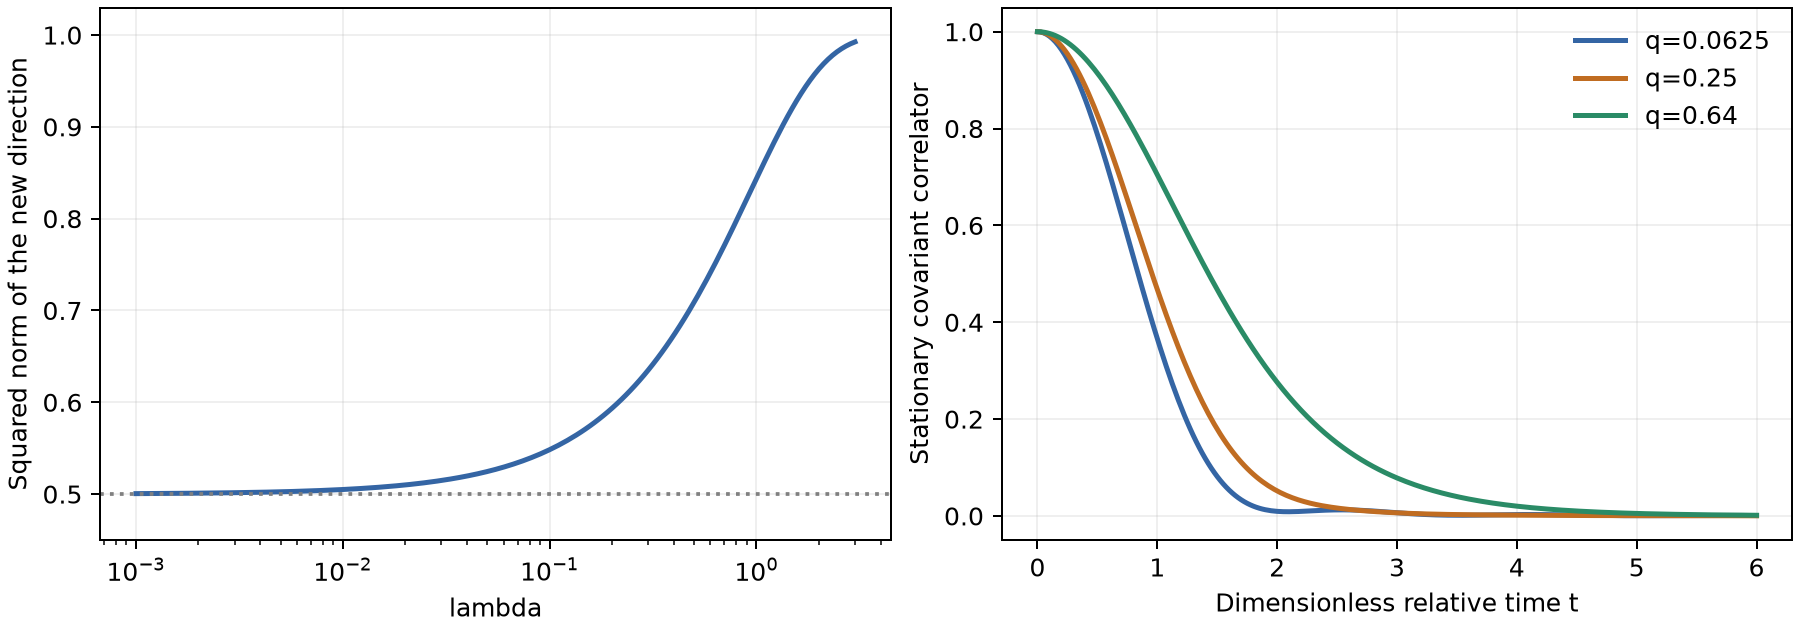
\includegraphics[width=\linewidth]{../../results/susskind-slater-covariant/covariant-channel.png}
\end{center}
\noindent The left panel plots \eqref{eq:residual}; the right panel
plots the stationary correlation. The physical examples use
$q=0.0625,0.25,0.64$ and $\lambda=-\log q/4$. The 18 saved time rows
use $t=0,0.5,1,2,4,6$, with Jacobi dimensions 80 and 120, and include
finite-difference curvature diagnostics. At $t=0$ the truncation
error is exactly zero; its logarithmic bound is stored as null.

\newpage
\section{Reproducibility, scope and the next microscopic task}
Three successful scientific runs were sealed before writing this
manuscript. No successful driver was rerun for presentation.
\begin{center}\small
\begin{tabular}{lp{10.1cm}}
\toprule
Output & Independent checks\\
\midrule
Site & 136704 exact CAR matrix comparisons at $(N,p)=(4,1),(4,2),(6,1)$;
7880 double-cluster coefficient checks through three edges.\\
Words & 8192 sixth words; 1458 old-restriction comparisons; 720 algebra
relations; 62 projection orthogonalities; 1638 Gram entries through
level three.\\
Spectrum & Three physical $q$ values, 18 time rows, 80/120 Jacobi
comparison, analytic cutoff bounds and curvature diagnostics.\\
\bottomrule
\end{tabular}
\end{center}
The exact word tests use rational $(\gamma,d)=(1/2,1/2),(2/3,1/2)$
as independent algebra parameters, with $c_U=-d\gamma$.
They are not points on the physical curve $q=e^{-4d^2}$.
Positive pivots in those finite Gram tests do not establish the
infinite positive representation; positivity above comes from the
microscopic limiting moments. The site checker independently applies
\begin{equation}
 2(p-\mathcal L)X=(2p-N)X+
 \sum_i(c_i^\dagger Xc_i+c_iXc_i^\dagger)
\end{equation}
and compares it with the marked-site construction. Numerical versions
are Python 3.14, NumPy 2.4.6, SciPy 1.18.0 and Matplotlib 3.11.0.
The stage manifest binds inputs, parameters, outputs, build logs and
page renders by SHA256. Floating diagnostics are not interval proofs.

The next task is the actual unpinched neutral-slope rank symbol and
selected-state control of pinching, followed by $J_2$ and the complete
bilocal in the common representation. The previously completed
full-trace bilocal four-point construction is an input, not an open
task to repeat. The spatial and mass generators, the de Sitter
temperature assignment and finite-$G$ dynamics remain to be derived.

\begin{thebibliography}{9}\small
\bibitem{BNR} M. Berkooz, P. Narovlansky and H. Raj,
\href{https://arxiv.org/abs/2006.13983}{arXiv:2006.13983},
version 2, Secs.~3.2--3.3 and 5.1.
\bibitem{EP} E. G. Effros and M. Popa,
\emph{Feynman diagrams and Wick products associated with $q$-Fock space},
\href{https://arxiv.org/abs/math/0303045}{arXiv:math/0303045}, Secs.~2--3.
\bibitem{RX} Rajgadia and Xu,
\href{https://arxiv.org/abs/2604.14387}{arXiv:2604.14387},
version 3, Secs.~4.1--4.2.
\bibitem{Ricard} E. Ricard, \emph{Factoriality of $q$-Gaussian von Neumann algebras},
\href{https://arxiv.org/abs/math/0311413}{arXiv:math/0311413},
version 2, Sec.~3, Theorem 1 and Corollary 2 (real dimension $\ge2$).
\bibitem{Xu} Xu,
\href{https://arxiv.org/abs/2403.09021}{arXiv:2403.09021},
version 3, Sec.~3.3, Eq.~(75).
\end{thebibliography}
\end{document}
